\chapter{Safe human-robot interaction: experimental results}
\label{chap:safety2}
\setfigurepath{figures/Safety2}
%=========================================================================
\begin{synopsis}
%In this chapter, we propose physically meaningful energy related safety indicators for robots sharing their workspace with humans.
%Based on these indicators, safety criteria are introduced as constraints in
%the control algorithm. The first constraint depending on the distance between the robot and the operator is placed on the kinetic energy
%of the robot to limit the amount of dissipated energy in case of collisions. A second
%constraint used to modulate contact forces is imposed on the amount of potential energy allowed to be
%generated within the human-robot system during physical contact. The control algorithm
%is formulated as an optimization problem and computes every time-step
%the needed actuation torques for a KUKA LWR4 manipulator given some task to
%be performed, the introduced constraints and the physical limitations of
%the system to cope with. The overall framework allows a human operator
%to safely enter the workspace of the robot and physically interact with it.
%ORIGINAL ABSTRACT
%In this chapter, the control strategy and energy related constraints introduced in the previous chapter are tested on a real KUKA LWR4 robot for interactions with a human-operator. As the person approaches the robot, the distance between the two is computed in real-time using a point-cloud based algorithm acquired with a set of depth sensors (Kinects). This distance is used to generate the constraint on the kinetic energy of the robot. At collision, dissipated energy and the resulting impact force are reduced.
%After establishment of physical contact, a second constraint is used to limit the amount of potential energy allowed to be generated within the human-robot system. Contact forces are saturated and the robot can safely be pushed or moved if needed. The overall framework allows a human operator to safely enter the workspace of the KUKA LWR4 and physically interact with it.
In this chapter, the controller and the energy related constraints introduced in the previous chapter are implemented and tested on a real KUKA LWR4 robot for physical and non-physical interactions with a nearby human-operator. As the person approaches the robot, the distance between the two is computed in real-time with an algorithm that uses point-clouds acquired from the scene by the mean of a set of depth sensors (Kinects). This distance is used to generate the instantaneous maximum amount of kinetic energy the robot is allowed to exhibit. At collision, thanks to the kinetic energy related constraint, dissipated energy and the resulting impact force are reduced. When physical contact between the KUKA LWR4 and the human is established, a second constraint is used to limit the amount of \textit{potential energy} that accumulates in the controller of the robot. Consequently, contact forces are saturated and the robot can safely be pushed and moved if needed. The overall control framework allows a human-operator to enter the workspace of the robotic manipulator, physically interact with it then safely leave its workspace.
%
%we propose physically meaningful energy re-
%lated safety indicators for robots sharing their workspace with humans.
%Based on these indicators, safety criteria are introduced as constraints
%in the control algorithm. The first constraint is placed on the kinetic
%energy of the robotic system to limit the amount of dissipated energy
%in case of collision. This constraint depends on the distance between the
%robot and the human operator. The distance is computed with a point
%cloud based algorithm acquired using a set of depth sensors (Kinects).
%The second constraint is on the amount of potential energy that is al-
%lowed to be generated within the human-robot system during physical
%contact. It is used to modulate the contact forces. The control algorithm
%is formulated as an optimization problem and computes every time step
%the actuation torques for a KUKA LWR4 manipulator given some task
%to be performed, the introduced constraints and the physical limitations
%of the system to respect. The overall framework allows a human operator
%to safely enter the robot’s workspace and physically interact with it.
%
%In this chapter, we propose physically meaningful energy related safety indicators for robots sharing their workspace with humans.
%Based on these indicators, safety criteria are introduced as constraints in
%the control algorithm. The first constraint depending on the distance between the robot and a nearby human operator is used to limit the amount of kinetic energy dissipated in case of a collision. After the establishment of physical contact, the second
%constraint is used to modulate contact forces by limiting the amount of potential energy generated within the human-robot system. The control algorithm
%is formulated as an optimization problem and computes every time-step
%the needed actuation torques for a KUKA LWR4 manipulator given some task to
%be performed, the introduced constraints and the physical limitations of
%the system to cope with. The overall framework allows a human operator
%to safely enter the workspace of the robot and physically interact with it.
\end{synopsis}
%=========================================================================
%=========================================================================
\section{Introduction}
\label{sec:experiment_on_kuka}
In the following sections, the experimental setup for the KUKA LWR4 robotic arm and the vision system used to detect the human-operator approaching and entering its workspace are described. A test case scenario is presented and the various reactions of the robot that can be induced using the safe controller presented in Chapter~\ref{chap:safety} along with the energy related constraints are discussed.
%%%%%%%%%%%%%%%%%%%%%%%%%%SECTION%%%%%%%%%%%%%%%%%%%%%%%%%%%%%
%%%%%%%%%%%%%%%%%%%%%%%%%%%%%%%%%%%%%%%%%%%%%%%%%%%%%%%%%%%%%%%%%
%%%%%%%%%%%%%%%%%%%%%%%%%%SECTION%%%%%%%%%%%%%%%%%%%%%%%%%%%%%
\section{Experimental setup}
The distance between the robot and the human-operator is computed using data from a set of 3 Kinect-like  depth sensors strategically placed around the workspace of the robot to avoid occlusions (see Fig.~\ref{fig:HR_INT_HW_STRUCT}). RGB and depth images from each sensor are calibrated and the pose of each device in the base frame of the robot is computed. The 3D model of the robot and the background  are removed from the depth images \cite{background_substraction} then  the pointclouds from the 3 depth sensors are down sampled and combined together. Finally the cluster of the human-operator is extracted from the resulting pointcloud \cite{PCL} and the minimum distance between the robot end-effector and the human-operator is computed and published via a ROS topic. The controller described in Section~\ref{subsec:cntrl_frmulation} of Chapter~\ref{chap:safety} is implemented as a C++ OROCOS \cite{rtt-url} component inside a generic software architecture developed at ISIR for robot manipulators  \cite{rtt-lwr-url}. The remote control PC runs a Xenomai kernel \cite{xenomai-url} with RTnet \cite{rtnet-url} to ensure minimum jitter in the real-time Ethernet communication. Finally, communication with the KUKA LWR4 Robot's Controller (KRC) is performed via the Fast Research Interface (FRI) \cite{schreiber2010fast}.
\begin{figure}
\centering
\captionsetup{width=.99\linewidth}\includegraphics[width=.99\linewidth]{\figurepath/HR_INT_HW_STRUCT}
\caption{View of a user sharing its workspace with a KUKA LWR4 robotic manipulator; with a schematic representation of the experimental setup used to measure the real-time distance between the robot and the human-operator and to control the robot.}
\label{fig:HR_INT_HW_STRUCT}
\end{figure}
%%%%%%%%%%%%%%%%%%%%%%%%%%SECTION%%%%%%%%%%%%%%%%%%%%%%%%%%%%%
%%%%%%%%%%%%%%%%%%%%%%%%%%%%%%%%%%%%%%%%%%%%%%%%%%%%%%%%%%%%%%%%%
%%%%%%%%%%%%%%%%%%%%%%%%%%SECTION%%%%%%%%%%%%%%%%%%%%%%%%%%%%%
\section{Test case scenario}
\label{subsec_test_case_scenario_2}
As a main activity, the robot performs a repetitive movement where it tracks a desired position on a straight line between two points \circled{A} and \circled{B}\footnote{Only when the end-effector of the robot reaches one point (e.g., \circled{A}) that the trajectory to the other point \circled{B} is generated.} in Cartesian space (see Fig.~\ref{fig:HR_INT_HW_STRUCT}). The controller described in (\ref{eq:ctrl_pbb}) is fed with a desired Cartesian position, velocity and a feed-forward acceleration term, and is implemented with the articular constraints corresponding to the physical limitations of the robot (\ref{eq:Constr_time_step})\footnote{As the real jerk capabilities of the actuators of the KUKA LWR4 are not known, the constraint on articular jerk (\ref{eq:cnt_lit_444}) is not considered in the version of the controller used for experiment.} along with the equality constraints described in (\ref{eq:dyn_eq_aab}) that correspond to its dynamic model. The LQP problem is solved for each period of time $\delta t = 15~ms$ to compute the needed control torque $\vect{\tau}_{|k}^{c}$. $\delta t$ is at the same time the \textit{sample-time} imposed to the controller and the \textit{time-window} used for the discrete formulation of the energy related constraints the robot must cope with. Fixed by trial and error , $\delta t = 15~ms$ is the least amount of time needed by the robot to be able to cope with the introduced (\textit{naively expressed}) energy related constraints: (\ref{eq:Safe_constr_1}) and (\ref{eq:Safe_constr_4}). In case $\delta t$ is fixed at $1~ms$, indeed, better tracking performances for the trajectory tracking task can be realized. However, with limited dynamic capabilities (i.e., producible deceleration and jerk in operational space), the system is incapable to react in time and cope (for example) with a constraint on its kinetic energy within just a  $1~ms$ time-window. When using such a small control sample-time, the energy related constraints must be reformulated to include the reaction capabilities of the robot. Exactly as have been realized for the constraints on articular position and velocity in Chapter~\ref{chap:Constrcomp} (see Section~\ref{sec:art_cnstr_new_frml}). Finally, the LQP is solved in real-time using Gurobi, a commercial optimization software \cite{gurobi}. 
%The robot's  movement is as dynamic as possible and the task is performed with the maximum needed kinetic energy to satisfy the desired $X^*$, $\dot{X^*}$ and $\ddot{X^*}$.
\begin{figure}[!ht]
\centering
\captionsetup{width=.99\linewidth}\includegraphics[width=0.99\linewidth]{\figurepath/e_p_xerr_sc_tau}
\caption{(a) Kinetic energy of the robot expressed at its end-effector in the direction of the human-operator. (b) \textit{Potential energy} stored in the controller of the robot during physical-contact. (c) Top: position tracking error. Middle: Reflected articular velocity constraint on the dynamic control variable (articular acceleration) of joint $0$. Bottom: Constrained articular velocity of joint $0$. d) Articular torques.}
\label{fig:e_p_xerr_sc_tau}
\end{figure}
The maximum tracking error for the position of the end-effector of the robot in Cartesian space is around $0.051~m$ (see Fig.~\ref{fig:e_p_xerr_sc_tau}.c Top). Such a large value is due to the activation of the constraint on articular velocity (\ref{eq:cnt_lit_tme_step_2}) that is reactively coped with as the velocity of joint $0$ reaches its max/min limits during the movements of the robot (see Fig.~\ref{fig:e_p_xerr_sc_tau}.c Middle). During the pre-collision phase, the maximum reached velocity of the end-effector is about $2~m/s$. When this movement is less dynamic, for example, with a maximum Cartesian velocity of $1~m/s$ instead $2~m/s$, the position tracking error for the robot end-effector can be reduced to  $0.005~m$. 
Note that the upper and lower limits for the velocity of this joint are fixed at lower values than what is recommended  by KUKA for the KUKA LWR4 robotic arm: $[\dot{q}_{m_{0}}, \dot{q}_{M_{0}}] = [-1.9, 1.9]~rad/s$ instead of $[-2.18, 2.18]~rad/s$. To explain this choice, note that the experiments presented in this chapter have been performed prior to our work on the \textit{constraints incompatibility} problem presented in Chapter~\ref{chap:Constrcomp}, it is therefore the classical formulations of the constraints related to the \textit{articular physical limitations} of the robot (\ref{eq:Constr_time_step}) that are hereby used in the configuration of the controller instead of the new formulations (\ref{eq:const_1_literature1}). Because of the uncertainties related to the dynamic model of the robot and the naive\footnote{Naive because they do not take into account the dynamic capabilities, i.e., the max/min deceleration and jerk producible by the actuators of the robot.} expressions of the constraints linked to its articular physical limitations, $\delta t$ for the discrete formulation of the joint velocity constraint (\ref{eq:cnt_lit_tme_step_2}) is fixed at $30~ms$ to give sufficient time to the system to react and saturate its articular velocity. 
%With the classic formulations, when fixing the control sample-time at $15~ms$, the system has been unable to properly cope with the imposed constraint on the velocity of joint $0$. Considering the highly dynamic movement of the end-effector, the robot within $15~ms$ is not able to deploy sufficient reaction capabilities (i.e., articular deceleration and jerk). This problem is resolved by increasing $\delta t$ for the discrete formulation of the joint rate constraint (\ref{eq:cnt_lit_tme_step_2}) to $30~ms$. When fixing  $\delta t$ for the joint rate constraint to such value, the system induces a braking movement that successfully saturates the velocity of the considered joint so the KUKA LWR4 Robot's Controller (KRC) does not trigger a ``\textit{joint velocity limit exceeded}'' error but results however into an inevitable exceeding of the imposed upper and lower limits $[-1.9, 1.9]~rad/s$ (see Fig.~\ref{fig:e_p_xerr_sc_tau}.c Bottom). This is mainly due to a drop in the precision of the \textit{discrete linearisation of the dynamics of the robot} that renders the control of its movement for a next time-step impossible to perform with the needed accuracy. Therefore, to prevent triggering a ``\textit{joint velocity limit exceeded}'' error, lower velocity limits have been chosen for the joint rate constraint. Clearly, all the problems related to this constraint can be avoided by using the new formulation of the constraint on articular velocity (\ref{eq:qddot_cond_to_satisfy_Jerk_Vel_compatibility_profile}) that has been introduced in Chapter~\ref{chap:Constrcomp} or simply by generating the needed trajectories for the robotic manipulator directly in joint space. 

%The maximum/minimum limits\footnote{The maximum/minimum limits on the articular velocity of the first joint are fixed in the QP at lower values than the real capacities of the robot.} on the articular velocity for the first joint are reached and violated. This is mainly caused by choosing $dt = 5 \cdot \delta t$ in (\ref{eq:const_15}). The reason for this choice and further explanations can be found in \cite{park1998enhanced}.
The maximum kinetic energy displayed by the robot in the direction of the nearby  human-operator\footnote{The direction of the human-operator is mainly along the $-\vect{x}$ axis (see Fig.~\ref{fig:HR_INT_HW_STRUCT}).} is $2.8~J$. $K_p$ is fixed at $200$ and $K_d = 28$.
%%%%%%%%%%%%%%%%%%%%%%%%%%SUBSECTION%%%%%%%%%%%%%%%%%%%%%%%%%%%%%
%%%%%%%%%%%%%%%%%%%%%%%%%%%%%%%%%%%%%%%%%%%%%%%%%%%%%%%%%%%%%%%%%
%%%%%%%%%%%%%%%%%%%%%%%%%%SUBSECTION%%%%%%%%%%%%%%%%%%%%%%%%%%%%%
\section[Human-robot interaction, scenario 1]{Scenario 1: human-operator intersecting with the trajectory of the robot and no constraints on its kinetic nor \textit{potential} energies}
In this case, the human-operator enters the workspace of the robot and intersects with its trajectory, a physical-contact is engaged and the movement of the robot is obstructed as it tries to reach its desired position towards point \circled{B}\footnote{The trajectory generator is blind to any collision with the environment. It continues generating desired position, velocity and feed forward acceleration for the end-effector of the robot.}. the controller is implemented as described in the test case scenario. No energy related constraints are considered. At collision (see video in \cite{kuka-url-noconstraints}), $2~J$ of kinetic energy are instantaneously dissipated to create the resulting impact force (see Fig.~\ref{fig:e_p_xerr_sc_tau}.a). \\
As shown in Fig.~\ref{fig:e_p_xerr_sc_tau}.b, after the establishment of physical-contact, \textit{potential energy} within the controller of the robot increases to reach a maximum value of $14~J$. We recall that this quantity is computed as: 
\begin{equation} 
S_{p_{contact}}^{x} &= m(\vect{q}_{|k})_{x}^{eq} \ddot{X}_{EE_{|k}}^{\vect{x}} \left(\vect{X}_{x_{|k}}^{*} - \vect{X}_{x_{|k}}\right) \vect{x},
\label{eq:hwcmputeEpx}
\end{equation}
with:
\begin{equation}  
\begin{split}
\ddot{X}_{EE_{|k}}^{\vect{x} & = \left(\dot{J}(\vect{q}_{|k})_{EE} \vect{\dot{q}}_{|k} + J(\vect{q}_{|k})_{EE} \vect{\ddot{q}}_{|k}^{c}\right) \vect{x} \\
\vect{\ddot{q}}_{|k}^{c}} &  =  M(\vect{q}_{|k})^{-1}\left(\vect{\tau}_{|k}^{c}-\vect{b}(\vect{q}_{|k},\vect{\dot{q}}_{|k})\right).
\end{split}
\label{eq:vefef_futur}
\end{equation}
Consequently, a contact force in the direction of the desired position is created. Generated articular torques can be seen in Fig.~\ref{fig:e_p_xerr_sc_tau}.d. We highlight the amount of torques in joint $0$ and joint $2$: $\tau_0 \simeq -18~N.m$ and $\tau_2 \simeq -16~N.m$\footnote{The contact force between the robot and the human-operator is mainly caused by the generated torques in joint $0$ and joint $2$. The contact force is not directly measured.}. Once  physical contact is released, the \textit{potential energy} stored in the system is transformed into kinetic one as fast as possible; which can be dangerous considering the nearby operator. Finally, the robot goes back to its normal behaviour. 
%%%%%%%%%%%%%%%%%%%%%%%%%%SUBSECTION%%%%%%%%%%%%%%%%%%%%%%%%%%%%%
%%%%%%%%%%%%%%%%%%%%%%%%%%%%%%%%%%%%%%%%%%%%%%%%%%%%%%%%%%%%%%%%%
%%%%%%%%%%%%%%%%%%%%%%%%%%SUBSECTION%%%%%%%%%%%%%%%%%%%%%%%%%%%%%
\section[Human-robot interaction, scenario 2]{Scenario 2: human-operator intersecting with the trajectory of the robot and constraint on its kinetic energy}
In this scenario, the human-operator gets within the workspace of the robot and intersects with its trajectory. As the person moves towards the robot, the first formulation of the constraint on kinetic energy (\ref{eq:Safe_constr_1}) is included\footnote{The constraint is not removed from the controller even after the establishment of physical-contact.} in the configuration of the controller and used to reduce the kinetic energy of the robotic manipulator before collision. We recall that this constraint has the following expression:
\begin{equation} 
S_c =  \frac{1}{2} m(\vect{q}_{|k})_{EE,O}^{eq} v_{EE_{|k+1}}^{{EE,O}^2} \leq E_{c_{limit}} = E_{c_{safe}} +  K (d - d_{safe}),
\label{eq:Safe_constr_11}
\end{equation}
Inequality and equality constraints used in the test case scenario are also considered in the control scheme. The parameters of the controller are fixed as: $E_{c_{safe}} = 0.02~J$ (if fixed at $0$, the robot stops moving), $K = 0.4~N$, $d_{safe} = 0.3~m$ and $d_{max} = 7~m$. As seen in Chapter~\ref{chap:safety} (Subsection~\ref{subsec:no_inter_constr_Ec}), choosing a big value for $K$ (e.g., $50$) will result in high articular jerks when the constraint on kinetic energy is activated (see Fig.~\ref{fig:tau3_qddot!!!!}.b). For this reason, a smaller value for $K$ is used when implementing the kinetic energy related constraint on the real robot. Also, a larger distance $(d_{max}-d_{safe}) = 6.7~m$ is allowed for the robot to reduce its kinetic energy. Compared to the braking distance used in simulation $(d_{max}-d_{safe}) = 0.2~m$.

Dissipated kinetic energy is shown in Fig.~\ref{fig:sc2}. At collision, only $0.02~J$ of energy are dissipated compared to the previous scenario in which the kinetic energy of the robot is not pre-constrained ($2~J$). As can be seen, the constraint is respected at every time-step and the impact between the robot and the operator is considered to be safe. We recall the safety limit value of dissipated kinetic energy recommended by the ISO/TS 15066 \cite{ISO15066PDF} standard in case of a collision between the robot and a human-operator at the level of the hands: $E_{c_{limit}} = 0.49~J$. \\
After the establishment of physical-contact, the non-constrained \textit{potential energy} starts accumulating in the controller of the robot to reach $\approx14~J$ (see Fig.~\ref{fig:e_p_xerr_sc_tau3}.a). Actuation torques of joint $0$ and joint $2$ that are directly proportional to the generated contact force are shown in Fig.~\ref{fig:e_p_xerr_sc_tau3}.b: $\tau_0 \simeq -20~N.m$ and $\tau_2 \simeq -17~N.m$. We highlight the chattering phenomenon on the actuation torque during physical-contact. Indeed, because of the inevitable occlusions, during this phase, the distance between the robot and the human operator is more difficult to compute and may become null. In this case, the constraint on kinetic energy can be released and consequently the robot forces its way towards point \circled{B} as its movement is obstructed by the human-operator. \\
After releasing physical-contact, the constraint on kinetic energy prevents the stored \textit{potential energy} from rapidly and dangerously transforming into kinetic one. The distance related constraint on the kinetic energy of the robot makes both the physical-contact establishment and releasing processes safer for physical human-robot interaction.  
%Fig Sc, Sp, tau
\begin{figure}[!ht]
\centering
\captionsetup{width=.99\linewidth}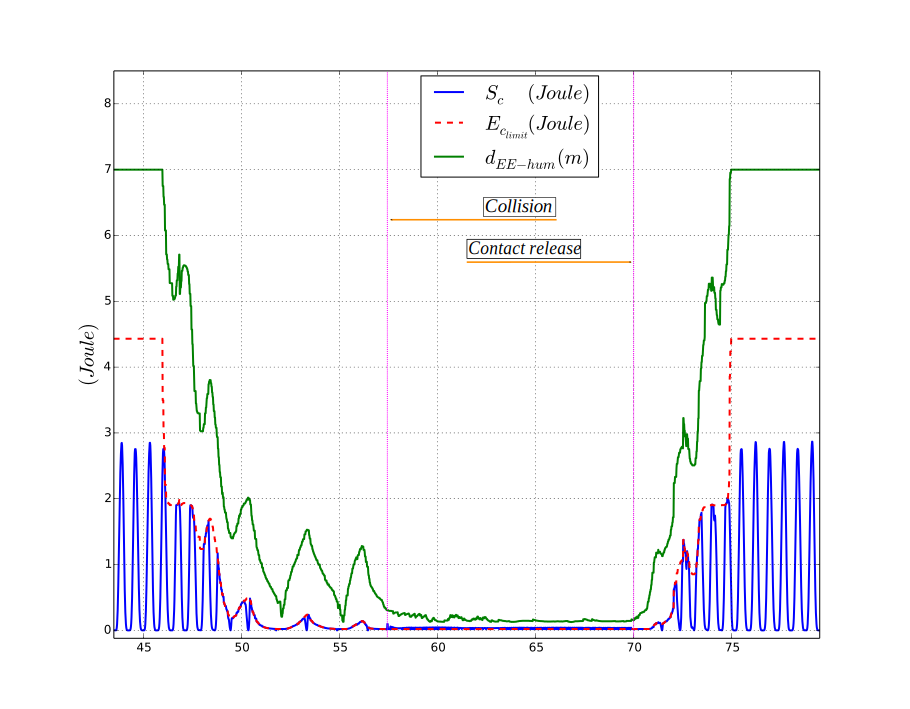
\includegraphics[width=0.89\linewidth]{\figurepath/sc2}
\caption{Constrained kinetic energy of the robotic manipulator expressed at the level of its end-effector in the direction of the approaching operator.}
\label{fig:sc2}
\end{figure}
\begin{figure}[!ht]
\centering
\captionsetup{width=.99\linewidth}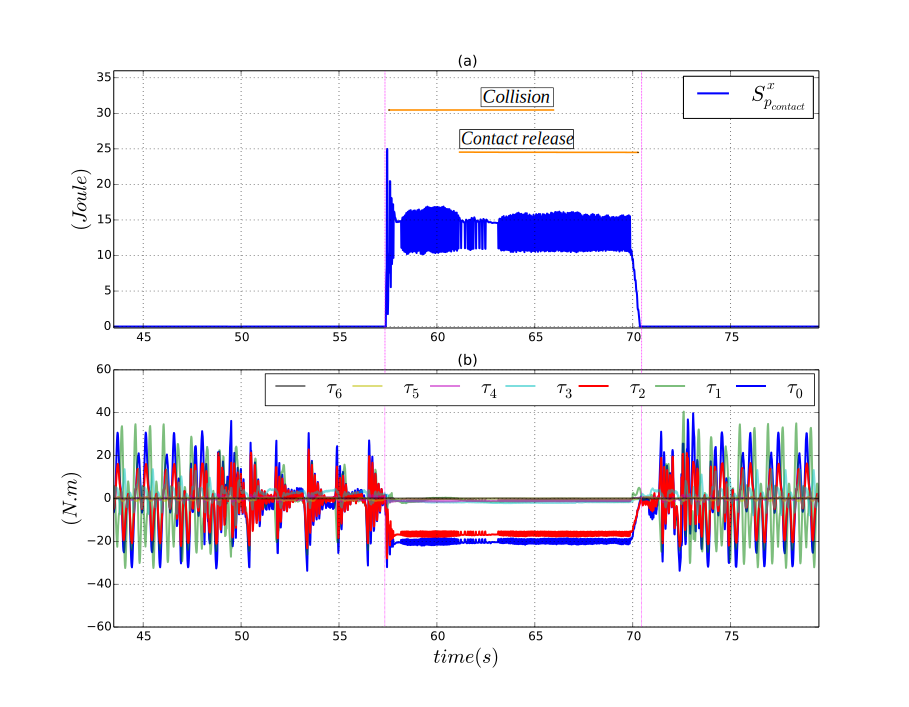
\includegraphics[width=0.99\linewidth]{\figurepath/e_p_xerr_sc_tau3}
\caption{(a) \textit{Potential energy} stored in the controller of the robot as it physically interacts with a human-operator within its workspace. (b) Articular torques.}
\label{fig:e_p_xerr_sc_tau3}
\end{figure}
%%%%%%%%%%%%%%%%%%%%%%%%%%SUBSECTION%%%%%%%%%%%%%%%%%%%%%%%%%%%%%
%%%%%%%%%%%%%%%%%%%%%%%%%%%%%%%%%%%%%%%%%%%%%%%%%%%%%%%%%%%%%%%%%
%%%%%%%%%%%%%%%%%%%%%%%%%%SUBSECTION%%%%%%%%%%%%%%%%%%%%%%%%%%%%%
\section[Human-robot interaction, scenario 3]{Scenario 3: human-operator intersecting with the trajectory of the robot and constraint on its \textit{potential energy}}
In this scenario, the person also intersects
with the trajectory of the robot between points \circled{A} and \circled{B}. The kinetic energy of the KUKA LWR4 is not constrained during the approach of the operator.
After the establishment of physical-contact, collision is detected using the system's proprioceptive torque sensors then, the constraint (\ref{eq:Safe_constr_4_3_axis54}) is added to the controller and used to limit the amount of \textit{potential energy} that accumulates in the controller of the robot. We recall the expression of such constraint:
\begin{subequations}
\label{eq:Safe_constr_4_3_axis1212}
\begin{empheq}[left={|S_{p_{contact}}^{\alpha}|=|m(\vect{q}_{|k})_{\alpha}^{eq} \ddot{X}_{EE_{|k}}^{\vect{\alpha}} \left(\vect{X}_{|k}^{*} - \vect{X}_{|k}\right) \vect{\alpha}| \leq  E_{p_{safe}}^{\alpha}\Leftrightarrow}\empheqlbrace]{align}
S_{p_{contact}}^{\alpha} &\leq \hspace{2.9mm} E_{p_{safe}}^{\alpha}, \label{eq:Safe_constr_4_x_axis_pos1212}\\ 
S_{p_{contact}}^{\alpha} &\geq - E_{p_{safe}}^{\alpha}, \label{eq:Safe_constr_4_x_axis_neg1212}
\end{empheq}
\end{subequations}
with $\alpha$ representing the $\vect{x}$, $\vect{y}$ and $\vect{z}$ axis in Cartesian space.
Except for the constraint on articular jerk, inequality and equality articular constraints described in (\ref{eq:Constr_time_step}) and (\ref{eq:dyn_eq_aab}) are also considered in the control scheme. The parameters of the controller are fixed as: $E_{p_{safe}}^{x} = 0.001~J$, $E_{p_{safe}}^{y} = 0~J$, $E_{p_{safe}}^{z} = 0~J$. 

At impact, as depicted in Fig.~\ref{fig:sc65}, $1.83~J$ of kinetic energy are instantaneously dissipated resulting into a more dangerous collision force, compared to the amount of kinetic energy ($0.02~J$) dissipated in the previous scenario. 
Fig.~\ref{fig:e_p_xerr_sc_tau657}.a shows how the constraint on \textit{potential energy} is satisfied at every time-step all along the physical-contact phase. Consequently, the contact force applied to the human-operator is harmless. Corresponding actuation torque and particularly of joints\footnote{The generated contact force during physical contact is mainly caused by the articular torques on these two joints.} $0$ and $2$ are shown in Fig.~\ref{fig:e_p_xerr_sc_tau657}.b: $\tau_0 \simeq -4~N.m$ and $\tau_2  \simeq -3~N.m$, compared to the two previous scenarios in which the constraint on \textit{potential energy} is not considered in the configuration of the controller: $\tau_0 \simeq -20~N.m$ and $\tau_2 \simeq -17~N.m$ during physical interaction. When using the introduced constraint on \textit{potential energy}, the robot is more compliant during physical-contact and if needed, can safely and easily be moved or pushed away by the human-operator. Also, thanks to this same constraint, no vibrations are induced by the actuators of the robot during physical-contact. 
\begin{figure}[!ht]
\centering
\captionsetup{width=0.99\linewidth}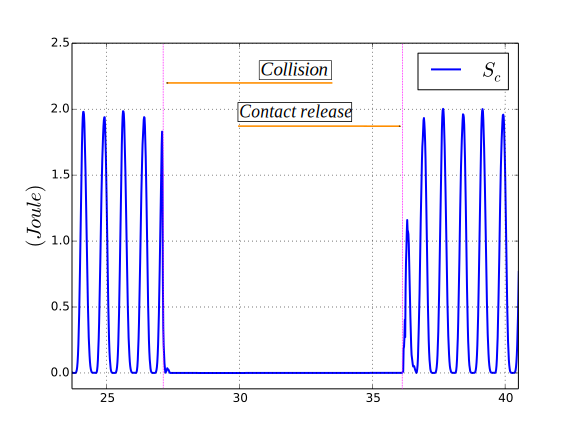
\includegraphics[width=0.80\linewidth]{\figurepath/sc65}
\caption{Kinetic energy deployed by the robotic manipulator expressed at the level of its end-effector in the direction of the human-operator entering its workspace and physically obstructing its movement.}
\label{fig:sc65}
\end{figure}
\begin{figure}[!ht]
\centering
\captionsetup{width=.99\linewidth}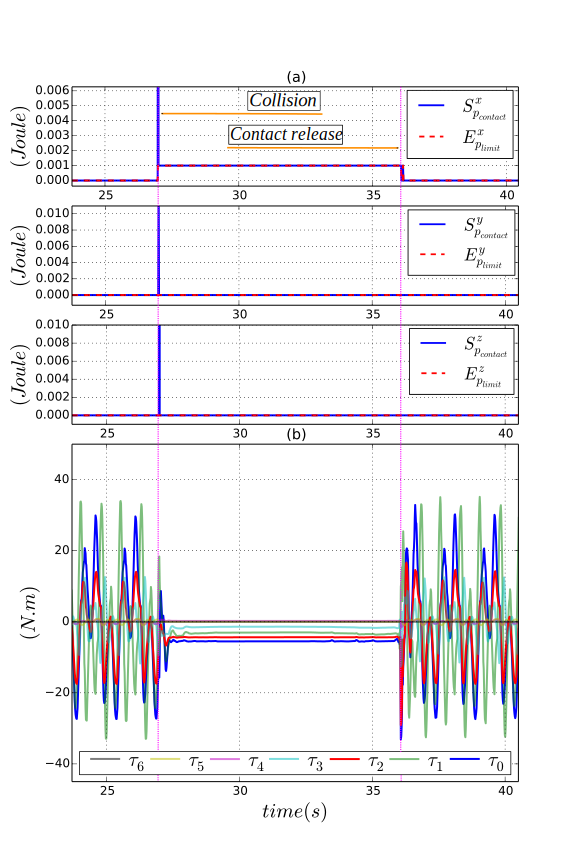
\includegraphics[width=0.89\linewidth]{\figurepath/e_p_xerr_sc_tau657}
\caption{(a) \textit{Potential energy} stored in the controller of the robot during physical contact along the $\vect{x}$, $\vect{y}$ and $\vect{z}$ axis in Cartesian space. (b) Articular torques.}
\label{fig:e_p_xerr_sc_tau657}
\end{figure}
Once contact is released, the constraint on \textit{potential energy} is de-activated and removed from the controller. Because of the accumulated position error\footnote{As the movement of the robot is retrained during-physical contact, the error between the real and desired positions for its end-effector accumulates and increases.}, at this stage, the controller of the robot holds a large amount of \textit{potential energy} $S_{p_{profile}}$\footnote{$S_{p_{profile}}$ is the \textit{potential energy} \textit{injected} in the controller of the robot at each time-step (see \ref{subsec:Task_energy_profile}).}. This energy transforms into kinetic one as fast as possible as the robot moves towards point \circled{B}. Because the  kinetic energy of the robot is not constrained, a harmful second collision is still possible with the nearby human-operator during this \textit{energy transformation} phase. Which makes the contact-releasing phase more dangerous, compared to the previous scenario in which the kinetic energy of the robot is constrained during the \textit{physical-contact release} phase. Finally, the KUKA LWR4 goes back to its normal behaviour.
%%%%%%%%%%%%%%%%%%%%%%%%%%SUBSECTION%%%%%%%%%%%%%%%%%%%%%%%%%%%%%
%%%%%%%%%%%%%%%%%%%%%%%%%%%%%%%%%%%%%%%%%%%%%%%%%%%%%%%%%%%%%%%%%
%%%%%%%%%%%%%%%%%%%%%%%%%%SUBSECTION%%%%%%%%%%%%%%%%%%%%%%%%%%%%%
\section[Human-robot interaction, scenario 4]{Scenario 4: human-operator intersecting with the trajectory of the robot and constraints on both its kinetic and \textit{potential} energies}
In this last scenario, the human also gets within the workspace of the KUKA LWR4 and intersects with its trajectory as the end-effector of the robotic arm tracks a desired trajectory between points \circled{A} and \circled{B} (see Fig.~\ref{fig:HR_INT_HW_STRUCT}). Using (\ref{eq:Safe_constr_11}), the kinetic energy of the robot is constrained during the approach of the operator. At impact, collision is detected using the system's proprioceptive torque sensors, physical contact is established then without removing the constraint on kinetic energy, the \textit{potential energy} related constraint (\ref{eq:Safe_constr_4_3_axis1212}) is added to the control scheme. This constraint is used to saturate the amount of \textit{potential energy} that accumulates in the controller of the robot along the $\vect{x}$, $\vect{y}$ and $\vect{z}$ axis in Cartesian space (see video in \cite{kuka-url-fullconstraints}). Except for the constraint on articular jerk, inequality and equality articular constraints described in (\ref{eq:Constr_time_step}) and (\ref{eq:dyn_eq_aab}) are also included in the configuration of the controller. Which parameters are fixed as: $E_{c_{safe}} = 0.06~J$, $K = 0.4~N$, $d_{safe} = 0.3~m$, $d_{max} = 7~m$, $E_{p_{safe}}^{x} = 0.001~J$, $E_{p_{safe}}^{y} = 0~J$ and $E_{p_{safe}}^{z} = 0~J$. 

As shown in Fig.~\ref{fig:sc6785}, the kinetic energy related constraint along the direction of the human-operator is respected at every time-step. At collision, only $0.02~J$ of kinetic energy is dissipated. Which results into a safe physical-contact establishment. During the post-collision phase, the constraint on \textit{potential energy} generated in the controller of the robot is also satisfied at every time-step (see Fig.~\ref{fig:e_p_xerr_sc_tau785}.a). This constraint is decoupled along the $\vect{x}$, $\vect{y}$ and $\vect{z}$ axis in Cartesian space and results into a reduced and safer contact force between the human and the robot. The KUKA LWR4 at this stage is compliant and can safely and easily be pushed or moved if needed. \\
Actuation torque of joint $0$ and joint $2$ that are directly proportional to the contact force are shown in Fig.~\ref{fig:e_p_xerr_sc_tau785}.b: $\tau_0 \simeq -4~N.m$ and $\tau_2 \simeq -3~N.m$, compared to the case when the constraint on \textit{potential energy} is not considered in the control scheme: $\tau_0 \simeq -20~N.m$ and $\tau_2 \simeq -17~N.m$ during physical contact. \\
\begin{figure}[!ht]
\centering
\captionsetup{width=0.99\linewidth}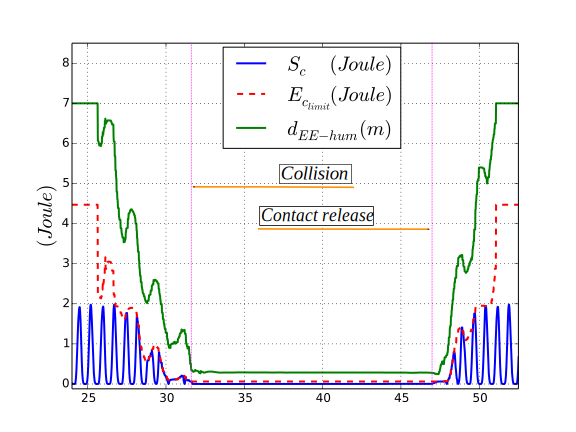
\includegraphics[width=0.89\linewidth]{\figurepath/sc6785}
\caption{Constrained kinetic energy of the robotic manipulator expressed at the level of its end-effector in the direction of the human-operator entering its workspace and physically obstructing its movement.}
\label{fig:sc6785}
\end{figure}
\begin{figure}[!ht]
\centering
\captionsetup{width=0.99\linewidth}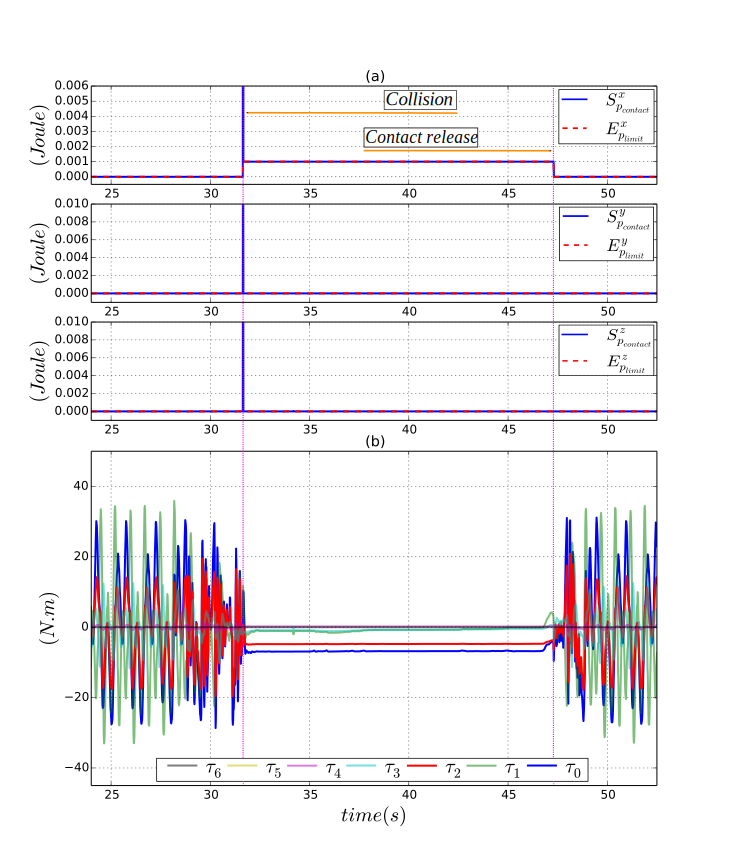
\includegraphics[width=0.89\linewidth]{\figurepath/e_p_xerr_sc_tau785}
\caption{(a) \textit{Potential energy} stored in the controller of the robot during physical contact along the $\vect{x}$, $\vect{y}$ and $\vect{z}$ axis in Cartesian space. (b) Articular torques.}
\label{fig:e_p_xerr_sc_tau785}
\end{figure}
Once contact is released, the constraint on \textit{potential energy} (\ref{eq:Safe_constr_4_3_axis1212}) is removed from the  configuration of the controller. At this moment, the robot contains sufficient \textit{potential energy} $E_{p} = m(\vect{q})_{EE,*}^{eq} \ddot{X}_{EE_{|k}}^{EE,*} \left(\vect{X}_{EE_{|k}}^{*} - \vect{X}_{EE_{|k}}\right) \vect{n}_{EE_{|k}}$ to move towards point \circled{B}. Considering the nearby operator who stills within its workspace, without the constraint on the kinetic energy of the robot, $E_{p}$ can rapidly transform into a hazardous amount of kinetic energy. however, thanks to the kinetic energy related constraint (\ref{eq:Safe_constr_11}), physical-contact is safely released and the \textit{potential energy} accumulated within the controller of the robot progressively and harmlessly transforms into kinetic one as the end-effector reaches its desired position \circled{B}.




  



%\subsubsection{Without constraints on kinetic and potential energy}
%\subsubsection{With constraints on kinetic and potential energy}

%
%
%\\
%Dissipated kinetic energy at collision is shown in Fig.~\ref{fig:dist_ec_ecmax_plot55}. As this energy is pre-constrained, only $0.035~J$ of kinetic energy are dissipated at collision; Resulting into an impact force of $85~N$ (see Fig.~\ref{fig:force_sensor255}).
%\begin{figure}[!htbp]
%\centering
%{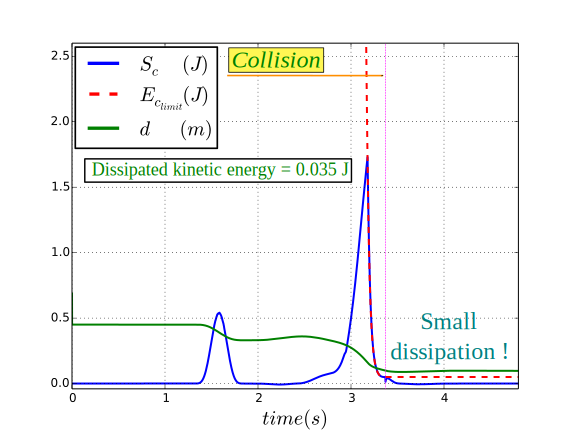
\includegraphics[width=0.8\columnwidth]{\figurepath/dist_ec_ecmax_plot55}}
%\caption{9} 
%\label{fig:dist_ec_ecmax_plot55}
%\end{figure}
%\begin{figure}[!htbp]
%\centering
%{\includegraphics[width=0.8\columnwidth]{\figurepath/force_sensor255}}
%\caption{10} 
%\label{fig:force_sensor255}
%\end{figure}
%As shown in Fig.~\ref{fig:dist_ec_ecmax_plot55}, the second formulation of constraint on the kinetic energy of the robot (\ref{eq:Safe_constr_2}) provides the  exact same results as when using the first formulation (\ref{eq:Safe_constr_1}) (see subsection \ref{subsec_inter_constr_Ec_classic}). It is respected at every time-step. As shown in (Fig.~\ref{fig:ep_contact_selon_x_seul_!!!!55}), during physical contact, the constraint on the potential energy generated within the robot-obstacle system is also respected at every time-step. 
%\begin{figure}[!htbp]
%\centering
%{\includegraphics[width=0.8\columnwidth]{\figurepath/ep_contact_selon_x_seul_!!!!55}}
%\caption{11} 
%\label{fig:ep_contact_selon_x_seul_!!!!55}
%\end{figure}
%Because this potential energy is saturated at a constant value of $0.1~J$, contact force as shown in (Fig.~\ref{fig:force_sensor255}) decreases over time to reach $0~N$\footnote{Physical contact is released.} when the desired position for the end-effector is diverging away from its real position. In case the physical contact is established with a human operator, the robot can be easily and safely moved or pushed away. This behaviour is actually the inverse of what happens without a constraint on the generated potential energy during physical contact. Potential energy increases and accordingly hazardous contact forces ( as shown in subsection \ref{subsec_no_constr_energy}). Fig.~\ref{fig:tau2555} shows the actuation torques of joint $0$ and joint $2$ that induce the braking movement for the end-effector when the constraint on kinetic energy is activated.  


%dire que c'est avantageux de pouvoir exprimer l'energie potentielle en n'importe quel point.
%\subsection{Simulation}
%\subsubsection{Test case scenario}
%\subsubsection{Kinetic energy modulation}
%\paragraph{Obstacle intersecting with the robot trajectory and no constraint on the kinetic energy}
%\paragraph{Nearby obstacle and constraint on the kinetic energy}
%\subsubsection{Contact forces and potential energy modulation}
%
%\subsection{Experiments on the real robot}
%\subsubsection{Test case scenario}
%\subsubsection{Without constraints on kinetic and potential energy}
%\subsubsection{With constraints on kinetic and potential energy}
%
%\section{Conclusion}



%%%%%%%%%%%%%%%%%%%FIGURES TRONQUEES SEPARES%%%%%%%%%%%%%%%%%%%

%%%%%FIGURES TRONQUEE GROUPEE%%%
%\begin{figure}[!htbp]
%\centering
%{\includegraphics[width=0.8\columnwidth]{\figurepath/collision_without_constr!!!!!}}
%\caption{9} 
%\label{fig:collision_without_constr!!!!!}
%\end{figure}
%%%%%FIGURES TRONQUEE GROUPEE%%%

%%%%%%%%%%%%%%%%%%%FIGURES NON TRONQUEES SEPARES%%%%%%%%%%%%%%%%%%%
%\subsection{1.1_COLLISION_WITHOUT_ANY_CONSTRAINT!!!!}
%\begin{figure}[!htbp]
%\centering
%{\includegraphics[width=0.8\columnwidth]{\figurepath/Ec_obst3!!!!}}
%\caption{9} 
%\label{fig:Ec_obst3!!!!}
%\end{figure}
%
%\begin{figure}[!htbp]
%\centering
%{\includegraphics[width=0.8\columnwidth]{\figurepath/force_sensor3!!!!}}
%\caption{10} 
%\label{fig:force_sensor3!!!!}
%\end{figure}
%
%\begin{figure}[!htbp]
%\centering
%{\includegraphics[width=0.8\columnwidth]{\figurepath/ep_contact_selon_x_seul3_!!!!}}
%\caption{11} 
%\label{fig:ep_contact_selon_x_seul3_!!!!}
%\end{figure}
%
%\begin{figure}[!htbp]
%\centering
%{\includegraphics[width=0.8\columnwidth]{\figurepath/tau3!!!!}}
%\caption{12} 
%\label{fig:tau3!!!!}
%\end{figure}
%%%%%%%%%%%%%%%%%%%FIGURES NON TRONQUEES SEPARES%%%%%%%%%%%%%%%%%%%

%\subsection{Nearby obstacle and constraint on the kinetic energy}
%In this case, a constraint on the kinetic energy of the end-effector is added to safely account for the presence of a considered obstacle. This constraint limits the actuation torque and, accordingly to (\ref{eq:S_2}), has a direct impact on the velocity of the end-effector. Depending on how the controller parameters values $d_{safe}$, $E_{safe}$ and $K$ are chosen, physical contact can be enabled or disabled.
%
%\subsubsection{Obstacle not intersecting the robot trajectory}
%In this scenario, the obstacle does not intersect with the path of the pick and place movement and the controller parameters are chosen as $E_{safe} = 0.01~J$, $k = 0.44~N.m$, $d_{safe} = 0.8~m$ and $d_{max} = 1.5~m$.
%\\
%In this particular case, the robot succeeds in achieving the pick and place movement but with a diminished dynamic performance compared to the unconstrained kinetic energy behaviour (see Fig.~\ref{fig:vel_track_wO_wpC_wEc}). Indeed, the constraint on the kinetic energy in the direction of the obstacle directly influences the velocity and the apparent inertia of the robot end-effector (2).   
% 
%%O:Obstacle, C:Contact, Ec:Energie cinétic, wp:withpossible   
%\begin{figure}[h]
%\centering
%{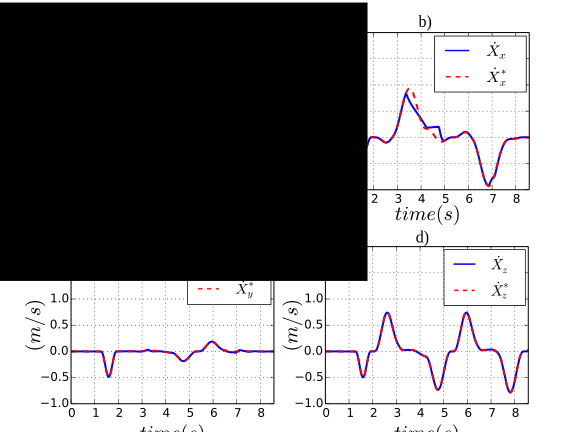
\includegraphics[width=0.7\columnwidth]{\figurepath/vel_wO_wpC_wEc}}
%\caption{a): Constrained kinetic energy of the end-effector in the direction of a nearby obstacle (case $O_2$ in Fig.~\ref{fig:kuka_in_xde}). b), c) and d): Influence of the constrained kinetic energy on the velocity performance for the  pick and place movement nearby the considered obstacle.} 
%\label{fig:vel_track_wO_wpC_wEc}
%\end{figure}
%
%The constraint on the kinetic energy of the end-effector in the direction of the considered obstacle (Fig.~\ref{fig:vel_track_wO_wpC_wEc}.a) is respected at every time-step and a drop in the velocity  can be observed in the $\dot{X}_x$ component (Fig.~\ref{fig:vel_track_wO_wpC_wEc}.b).
%
%
%\subsubsection{Obstacle intersecting the robot movement}
%In this scenario, the obstacle intersects with the \circled{2}-\circled{3} segment of the pick and place movement trajectory and the controller parameters are taken as  $E_{safe} = 0.01~J$, $k = 0.44~N.m$, $d_{safe} = 0.8~m$ and $d_{max} = 1.5~m$. The kinetic energy of the end-effector during the collision phase is shown in Fig.~\ref{fig:kE_wO_wC_wEc}.
% 
%\begin{figure}[h]
%\centering
%{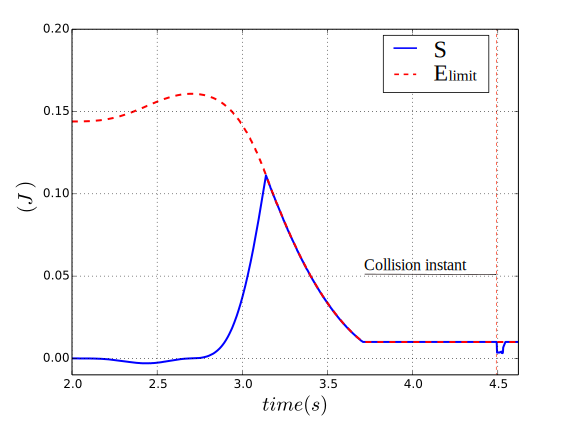
\includegraphics[width=0.6\columnwidth]{\figurepath/kE_wO_wC_wEc}}
%\caption{Dissipation of the constrained kinetic energy of the end-effector in the direction of the considered obstacle during a collision phase.} 
%\label{fig:kE_wO_wC_wEc}
%\end{figure}
%
%The kinetic energy profiles of the two collision phases in Fig.~\ref{fig:kE_wO_wC_wEc} and 7 show the benefit of using the safety criterion introduced in (3). Indeed, the dissipated energy when the kinetic energy of the end-effector is initially constrained is less than the dissipation without any constraint. This particular property of the presented controller allows safer physical interactions between the robot and its environment.   

%\subsection{Ep profile all the time with contr on Ec withEp the constr are compatible}
\section{Conclusion}
\label{sec:safety2conclusion}
In this chapter, the controller and energy related constraints introduced in Chapter~\ref{chap:safety} have been successfully implemented on a real KUKA LWR4 robot as it physically interacts with a human-operator. As the person approaches the robot and enters its workspace, using the kinetic energy related constraint, the kinetic energy displayed by the robotic arm in the direction of the human-operator is saturated. The robot still performs its assigned task but with a diminished dynamics. Physical-contact can then safely be established. \\
During the post-collision phase, the \textit{potential energy} that accumulates in the controller of the robot is also successfully constrained. Depending on the allowed amount of \textit{potential energy}, the resulting contact force can be reduced and if needed, the robot easily and safely moved by the operator. \\
After releasing physical-contact, the constraint on kinetic energy ensures a smooth and safe transformation of the \textit{potential energy} held in the system's controller into kinetic one. Consequently, the human-operator can safely and progressively leave the workspace of the robotic manipulator. The task dynamical performances of the robot are then fully recovered. 

As explained in Chapter~\ref{chap:Constrcomp} and Chapter~\ref{chap:safety}, a solution to the control problem cannot be guaranteed for every time-step if the formulations of the introduced energy related constraints do not take into account the reaction capabilities\footnote{i.e., producible articular torque/deceleration and jerk.} of the actuators of the robot. This is actually the reason why the control sample-time for the implementation of the introduced energy related constraints on the real robot is increased from $1~ms$ in simulation to $15~ms$ in the real life. The KUKA LWR4, for example,  is not able to brake and cope with $E_{c_{limit}}$ within only $1~ms$ of time-window and $15~ms$ is the smallest duration needed for the robot to cope with the limit of the kinetic energy related constraint. Moreover, increasing the control time-step duration deteriorates the tracking performances of the robot regarding the trajectory tracking task it has to perform. \\
The only way to guarantee the existence of a solution to the control problem for every time-step is to reformulate the energy related constraints to include the max/min producible articular torque/deceleration and jerk. However, because of the dynamical and non-predictable nature of $E_{c_{limit}}$ in (\ref{eq:Ec_constr_a}), ensuring the \textit{viability} of the state of the robot during human-robot interaction is even more difficult. Indeed, $E_{c_{limit}}$ depends on the non-predictable movements of the human-operator and  on his real-time distance to the robot. The constraint on the kinetic energy displayed by the robot is therefore of type 6 (see table \ref{my-label} in Chapter~\ref{chap:Constrcomp}) and can be modified as follows. Similarly to the joint velocity constraint: $\vect{\dot{q}}_{|k} \leq \vect{\dot{q}}_{M}$, $S_c \leq E_{c_{limit}}$ can be written: 
\begin{equation}
v_{|k+1} \leq \sqrt{\frac{2 E_{c_{limit}}}{m(\vect{q}_{|k})^{eq}}},
\label{eq:dyn_Ec_cnstr}
\end{equation}
with $\~v_{limit} = \sqrt{\frac{2 E_{c_{limit}}}{m(\vect{q}_{|k})^{eq}}}$ being a dynamic limit in contrast to $\vect{\dot{q}}_{M}$ which is a static limit. To ensure at every time-step a solution to the control problem when the system must cope with such a constraint on its kinetic energy, (\ref{eq:dyn_Ec_cnstr}) can be reformulated as:
\begin{equation}
v_{|k+n} =  v_{|k} + n \ddot{X} \delta t + \frac{(n^{2}-n)}{2} \dddot{X}_{m} \delta t^2 \leq \~v_{limit}^{predicted},
\label{eq:dyn_Ec_cnstr2}
\end{equation}
with $\ddot{X}  = \dot{J}(\vect{q}_{|k}) \vect{\dot{q}}_{|k} + J(\vect{q}_{|k}) \vect{\ddot{q}}_{|k}^{c}$, $n$ the maximum number of time-steps needed for the robot in a state $S_{|k}$ to bring its acceleration expressed in operational space to $0$ considering a constant amount of jerk $\dddot{X}_m$ it can produce.  $\~v_{limit}^{predicted}$ is the predicted value of $\~v_{limit}$. The main challenge then is to properly compute $n$ and the prediction horizon $p$ for $\~v_{limit}^{predicted}$:
\begin{equation}
\~v_{limit_{|k}}^{predicted} = \~v_{limit_{|k}} + p \ddot{X}_m,
\label{eq:dyn_Ec_cnstr222}
\end{equation}
with $\ddot{X}_m$ the maximum variation of $v_{|k}$ in operational space the robot can handle. Finally, note that when using the formulation of the constraint on the  kinetic energy (\ref{eq:dyn_Ec_cnstr2}) that takes into account the dynamic capabilities of the actuators of the robot, the control sample-time in theory may potentially be fixed at $1~ms$ without causing any \textit{constraints incompatibility} problems. 


%The energy based safety indicators presented in this chapter allow a continuously safe human-robot interaction.  It allows the robotic system to adapt its dynamic behaviour from the approach of the human operator to the establishment of physical contact. Contact and impact forces are modulated all along the interaction process and the contact enabling/disabling transition is smoothed thanks to the universality of the energetic formulation. 


